\documentclass[12pt,a4paper]{article}
\usepackage{times}
\usepackage{durhampaper}
\usepackage{harvard}
\usepackage{graphicx}
\usepackage{longtable}
\usepackage{siunitx}

\citationmode{abbr}
\bibliographystyle{agsm}

\title{Enigma and BOMBE simulation}
\author{A.L. Gillies}
\student{A.L. Gillies}
\supervisor{M. Johnson}
\degree{MEng Computer Science}

\date{}
\begin{document}
\maketitle

\begin{abstract}\\

{\bf Context/Background} - The Enigma and BOMBE formed the basis of communication throughout the Axis powers. Technology has advanced since then, but how much? This will be the foundation of this paper, how much faster are we now, than then?\\

{\bf Aims} - Using the known execution speed of the antique Enigma and BOMBE, the aim of this paper is to show, through implementation and testing of a modern interpretation of the Enigma and BOMBE, the magnitude of speed up that has occurred since the inception of both.\\

{\bf Method} - Both machines have been re-created using modern technology and techniques, they have been timed, and this measurement will be compared to the same measurement on the original machine.\\

{\bf Results} - The modern versions of both are far faster than their antiquated counterparts. The magnitude of which can be seen in the results section.\\ Needs more \\

{\bf Conclusions} - The significant leaps that have been made in computing in the last 70 years cannot be overstated, The development from electro-mechanical devices to the silicon based computers we have today are astounding.
\end{abstract}

\begin{keywords}
Enigma, BOMBE, Parallel, Modern, Computation, Evaluation, Reinterpretation, Comparison, C++, Antiquated.
\end{keywords}



\section{Introduction}

\iffalse
What the project is about - talk through the motivations and a rough outline of the project\\
The project aims to show that a significant speed up has occurred in the field of computation since the inception of this cryptographic technique.
Context of the project - what are some real world things that need to be taken into account\\
What was achieved - go through deliverables and then go through issues and counter\\
2-3 pages\\
\fi

Since the time of Alan Turing, the developments of computational power cannot be understated. We have developed from electromechanical devices that have a single function, to electronic devices that are capable of renders and simulations of electromechanical devices within themselves, the BOMBE is an example of an electromechanical device and this can be rendered and simulated within a modern mobile device, let alone the cutting edge, which at the time, the BOMBE was. Within more cutting edge technology we are able to study models of the universe, and other academic pursuits that were inconceivable at the time of Alan Turing.\\

Alan Turing is the man that is credited with the creation of the BOMBE, this electromechanical device is then credited with breaking the German Enigma codes that are encrypted using the Enigma machine, this is another electromechanical device with a single function, it is used to encrypt messages that are then sent to another enigma machine that will then encrypt the message. This is how almost all of the German orders were relayed. The breaking of this code is said to have shortened the second world war by several years and thus save innumerable lives.\\

The motivations of this project are two fold, the first is to show the effectiveness of both the Enigma machine and the BOMBE. This will be done via the implementation of both in a modern setting. The second is to outline the developments that have occurred since the inception of the Enigma and BOMBE, by showing the significant increase in computational efficiency, an analogue for this would be how fast the BOMBE breaks the Enigma code. The most simple solution will be a BOMBE representation using modern coding techniques without any parallel improvement or any other modern techniques. This will be purely a copy of the enigma, in C++ code. This will outline the improvements between an electromechanical device and the sequential electronic devices that have been common from around the 1980s. The second, more complex solution will incorporate parallel programming, this was introduced in the early 21st century, and is still an improving technology.\\

\subsection{Deliverables}

\label{units}
\begin{longtable}{ |p{1.25cm}|p{4cm}|p{7cm}| }\hline\hline
Unique ID & Deliverable & Description \\ \hline
DL1 & Simulate the Enigma Machine & Have a working Enigma machine that can take in settings and plaintext and return ciphertext. \\ \hline
DL2 & Simulate the Bombe & A working BOMBE that takes in settings and ciphertext and returns decoded plaintext. \\ \hline
DL3 & Show the correctness of the Enigma Machine & Show through a series of tests and validations that the plaintext fed to the Enigma Machine and the Ciphertext returned are paired through the settings of the enigma \\ \hline
DL4 & Show the correctness of the BOMBE & Show that the known plaintext of the ciphertext input into the BOMBE is exactly the same as the plaintext that is returned by the BOMBE \\ \hline
DL5 & Evaluate average computation time over set inputs for both Enigma and BOMBE & Using a wide range of known plaintext - ciphertext pairs find the average computation time, the time take on average to do a single encode or decode for both simulations \\ \hline
DL6 & Parallelise The BOMBE and evaluate average computation time & Using known parallelisation techniques increase the speed at which the BOMBE will decode a given ciphertext \\ \hline
\end{longtable}

\section{Related Work}

\iffalse
Survey relevant literature\\
Relate to your own project\\
This should contain all details of the OG BOMBE and Enigma\\
May be able to reuse parts of the literature survey\\
use anything relating to parallel computing, the introduction of common single core computing, the introduction of C++ code, the development of the intel tool set, any historical papers about the enigma code, anything about the BOMBE, anything about the measurement of computational improvements.\\
2 pages\\
\fi

The electromechanical device known as the Enigma machine is best known for its use by the Third Reich, it was first designed by a company called Scherbius \& Ritter in 1918, and then sold to the German armed forces, after a few incremental upgrades. The machine is designed to allow secure cryptographic messages between two of these machines, the first will encode the message using decided settings, the second will, using the same setting, decode the message. This is done through a set of alphabet mapping, a one to one relationship between one alphabet and another, one letter is mapped to another and this relationship is bidirectional. No two letters from one alphabet map to the same letter in another.\\

The Enigma machine is made up of 7 parts, there are only 5 important parts plus an additional component and some wiring to make it work. The important parts are the plug-board, the three rotors, and the reflector. The other parts are a converter that allows all the separate components to work together, along with a lamp-board to show the encrypted letter, along with wiring to connect them all together.\\

The plug-board is a mapping from one alphabet to another that is a manual process of re-plugging 26 wires that map from one to the other. This does not change for each letter that is input into the device, unlike some of the components we will see later. The reflector is much the same as the plug-board, except that it cannot map a letter to itself. It is a simple one to one mapping that does not change over time, in the earlier designs of the Enigma machine, it could not be rewired, and instead had to be swapped out for another reflector with different wiring, in a similar way to that of the rotors that we discus later on, with later designs came the ability to rewire it. The rotors are the core of the machine. These are three modular, circular, mappings that are altered each time a letter is encrypted by the machine. The way they work is that the inner ring and outer ring each have contacts on them, when the outer ring is rotated then the mapping will change. there are 26 different mappings that can be used. The three rotors are chosen from a set of available rotors and each one has a unique ordering of letters on both its rings. Thus the order in which the rotors are input into the machine is important.\\

The enigma machine will take the first letter of the message that is to be encrypted from a keyboard and first pass it through the plug-board, it will then go to a converter which allows the signal to be passed to the first rotor, another mapping, then the second, and the third, in each of these case the inner ring of the previous rotor is connected to the outer ring of the next rotor. Then the reflector is reached, the mapped letter is then passed to the inner ring of the third rotor and this is a reverse mapping. The outer ring of the third rotor is connected to the inner ring of the second rotor and thus the signal will pass back through the rotors in this fashion. Once the plug-board is reached, the reverse mapping is done and a light will trigger on the lamp-board showing the letter that the input letter has been mapped to. After this the rotors are then stepped, this means that the first rotor will rotate one position for each letter that is encrypted. The second rotor will only step when specific notches are reached on the first rotor, the third is the same but for notches on the second rotor. Based on this method the first rotor will rotate more than the second and the second will rotate more than the third.\\

The BOMBE developed at Beletchly Park was very similar to the Enigma, but its antithesis. The BOMBE was based on a probably phrase attack, this means that for the BOMBE to work there needs to exist a known or guessed portion of ciphertext and its corresponding plaintext. An example of this that was used regularly was the German equivalent of "Weather Report", this was done daily and could easily be guessed. Once this was established then the exact letter to letter transformation must be established, this is done through the matching of letter to letter in the phrase such that no letter is encoded as itself as this is impossible for the enigma. Examples of these matching shown in figure 1.

\begin{figure}[h]
\centering
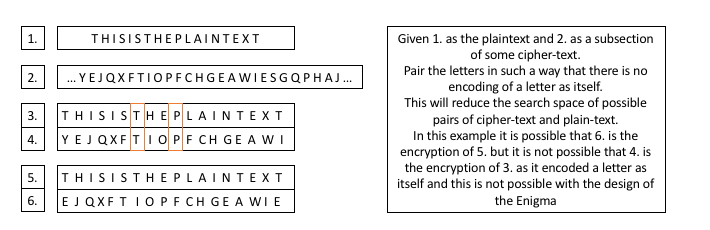
\includegraphics[width=\textwidth]{StageOneBOMBE.png}
\end{figure}

The next stage of preprocessing is the creation of crib-ciphertext pairings. This is the mapping of a specific letter at a specific set up of the enigma. For example in the figure above we can see that T maps to E at the first set up of the Enigma, at the second set up of the Enigma, because due to the rotor stepping we are now in a different set up, H maps to J, and so on. These pairs can then be joined to create a graph of pairings with the numbered setting as a label for the edge, a random example is shown in figure 2.

\begin{figure}[h]
\centering
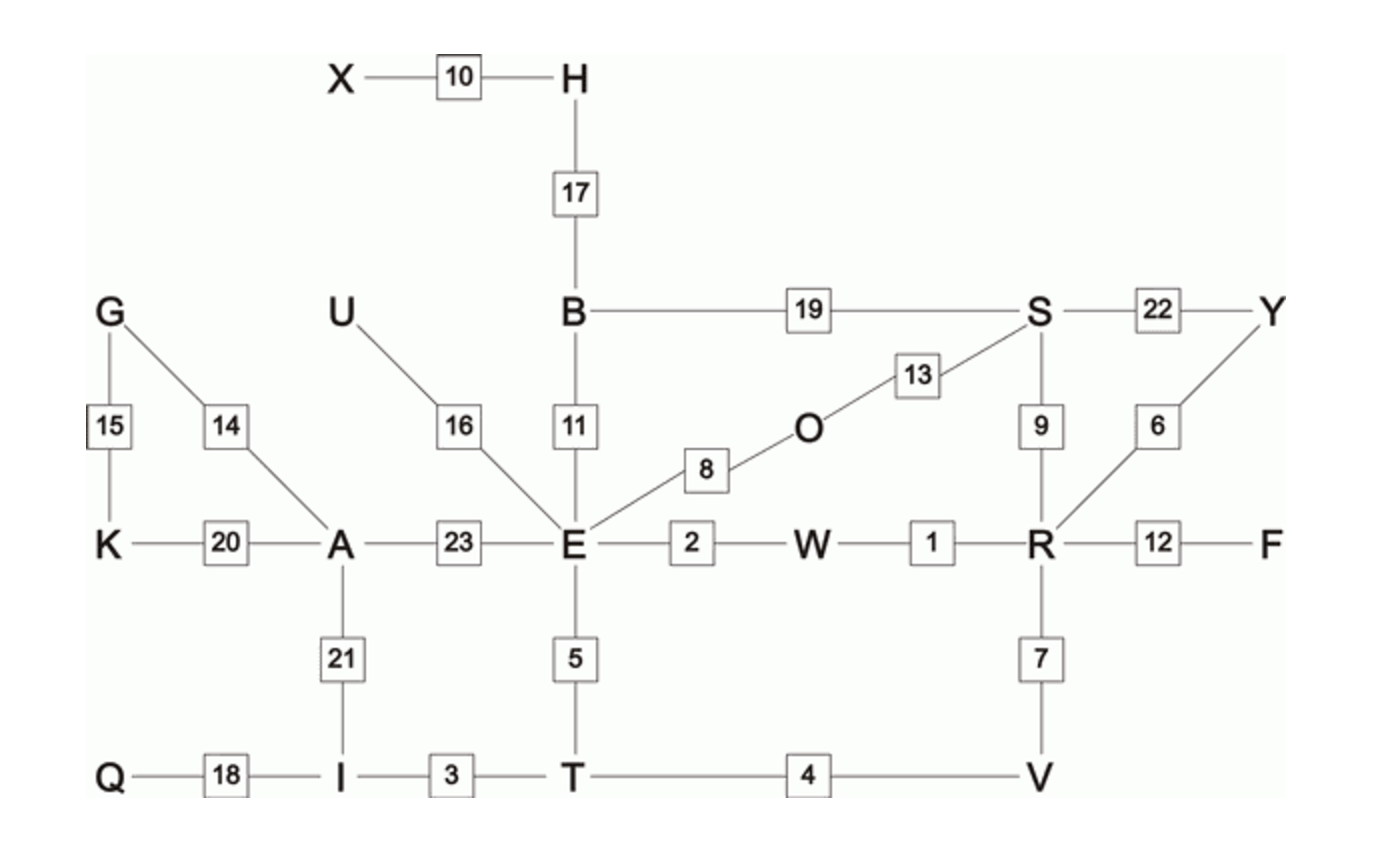
\includegraphics[width=\textwidth]{StageTwoBOMBE.png}
\end{figure}

There are significant implications that can be drawn from the connection network, the graph of pairings in figure two. Using the connection network the search space can be reduced by using the implications of some transformations on others. We first must recall that each transformation consists of two 'stecker swappings' and a 'scrambler encryption' these are the set of rotor transformation and reflector respectively. A 'stecker swapping' is the transformation of a letter through use of the three rotors that are present in the enigma, a 'scrambler encryption' is the transformation via the reflector, and then another 'stecker swapping' is the use of the reverse direction of the rotors. A relative position is the numbered set up that the enigma is currently in, so the first letter input into the enigma machine is using relative position 1, which is simply a set up of the enigma, relative position two is the set up of the enigma given that a letter has already been input and that the set up has changed due to the way the rotors behave. Using the connection network above, here is an example of the search space reduction that can be done using these details.\\

For example, let us test the hypothesis that E is mapped to K through the first three rotors, also known as E is "steckered" to K. Now consider how E is transformed into A at relative position 23, this is shown on the connection network above.

If E is "steckered" to K, K will be input to the reflector or "scrambler" at relative position 23 which will output some other letter L1. Since we know that E transforms into A at relative position 23, we know that A must be "steckered" to L1.

But if A is "steckered" to L1, L1 will be input to the "scrambler" at relative position 21 which will output some other letter L2. Since we know that A transforms into I at relative position 21, we know that I must be "steckered" to L2.

But if I is "steckered" to L2, L2 will be input to the "scrambler" at relative position 3 which will output some other letter L3. Since we know that I transforms into T at relative position 3, we know that T must be "steckered" to L3.

But if T is "steckered" to L3, L3 will be input to the "scrambler" at relative position 5.

Now consider the output of the "scrambler" at relative position 5 when it receives L3 as its input. Since we know that T transforms into E at relative position 5, we know that the output letter of the "scrambler" at relative position 5 must be "steckered" to E.

Suppose, when given L3 as its input, the "scrambler" at relative position 5 outputs J. By our original hypothesis E is "steckered" to K, but by our chain of implications E is "steckered" to J, so in this case E is "steckered" to both K and J. But the construction of the Enigma does not permit one letter to be "steckered" to two letters, so E cannot be "steckered" to both K and J, so our original hypothesis has resulted in an impossible consequence and so must be false.

But now suppose, when given L3 as its input, the "scrambler" at relative position 5 outputs K. Then by our original hypothesis E is "steckered" to K, and by our chain of implications E is "steckered" to K, so in this case E is "steckered" only to K, thus our original hypothesis has resulted in a consistent consequence and so may be true.

The altered connection network bellow shows the hypothesis that E is "steckered" to K via the the steps of implication that we have been through.

This is the way that the preprocessing that was done helped reduced the search space that it would have to be iterated through by the BOMBE and thus reducing the time taken for a result to be found.

The way the electro-mechanical device was created is very similar to an exploded view of the Enigma, it was created so that there would be no return journey through the rotors, instead another three rotors were added after the reflector. They were added in such a way that one pass through these 7 components is the equivalent of a pass through to the reflector and back through the rotors of the Enigma. The BOMBE was made up of three batteries of 12 sets of these 7 components. With the use of a "menu", also known as the connection network, this monstrous machine could be wired up so as to eliminate as many combinations as possible.

There may be a bit of confusion at this point, the question, "Where has the plug-board gone?" may be asked. This has been removed as it does not change throughout the use of the machine, the same is said of the reflector but this would  be very hard to remove in the same fashion as has been left. The reason that the plug-board can be removed so easily is that is can be easily defeated by frequency analysis, this is the process of matching letter frequencies between the language of the plaintext and the language of the ciphertext, an example; the letter E make up a third of all letter in the plaintext language, the letter R makes up a third of the ciphertext messages, we can therefore assume that E has been transformed to R by the plug-board, this is done for all letter of the plaintext language and with some intuition as to the native language the messages have been sent in, the plaintext can be retrieved. 

\section{Solution}

\iffalse
Overview of architecture and design - use parts from the design report\\
Description of tools used - design report\\
Outline of algorithms to be used - design report\\
Features of the implementation process - issues and struggles with the implementation, how they were overcome\\
Testing - validation and all other testing done\\
Verification and validation\\
Stages of the life cycle undertaken - software engineering\\
4-7 pages\\
\fi

\subsection{Enigma}

C++ was chosen as the implementation language for the enigma mainly due to its rich library, it has support for a wide range of external libraries, the main one we will be focused on in this case is the Intel tool set, this may not be much use when it comes to the Enigma but it is a very strong and well established tool that allows C or C++ code to be parallelised which is the aim of the BOMBE implementation that will be outlined later. The reason that C++ was chosen specifically for the Enigma implementation is that it is a middle level language and thus enables the benefits of low level and high level languages as well as being highly portable and non operating system specific. It is also very well established in the teaching at Durham University.\\

The recreation of the enigma machine was to be done in C++, this was chosen as it has significant parallel tools available for it, in the form of the Intel c++ compiler. A tool that has shown great capabilities in parallelism. This would be very helpful in the creation of the advanced BOMBE recreation and developing in two separate languages didn't make sense.\\

The recreation revolves around a settings file, this is a text file that contains all the setting that will be used by the enigma machine to encode the message that it is given through the command line interface, these settings include; the plug-board mapping, the reflector mapping, the rotors that will be used and their corresponding initial displacement. This file is then updated automatically to reflect the changes that have occurred to the settings as the message is encrypted, each letter will have a different set of setting as the displacement of the rotors changes, this will be reflected in the settings file. The c++ file that makes up the core of the code that has realised enigma, is called the main file, this will manage all the changes that occur as well as managing user interaction with the device and having a central location with which to manage the other c++ files that realise different parts of the enigma machine.\\

The plug-board, reflector, rotors, as well as a converter file have all been created in their own separate files so as to improve the modularity of the system, as well as provide a more focused development route; each file can be developed without removing functionality for the others.\\

The main file contains the instructions on how to use the system, it contains all file dependency instructions, as well as containing the set up function and main function. The set up function will be run before the system is usable, it will find the set up file, using the information that it contains, it will then make the system usable through the main function of the main file. As the set up function is run, it will call the set up functions of all the other parts of the enigma in other files, the plug-board file will store its mapping, the reflector will store its mapping and the rotors file will store the rotors that are currently in use and make sure that the displacement is correct for each one. Once this has been done the main function is used, this will take in user input through the command line, the only thing that will be input is the plaintext, this is the message to be encrypted. The main file will then iterate through each of the letter in the message and encrypt them individually, using unique settings for each letter. The first letter will use the settings that have been read in by the set up file. the first stage is to convert the letter to its corresponding number, for example A is equal to 1 and Z is equal to 26, this makes use of the converter file, this file contains functions to convert between letters and numbers as well as another function that does the reverse. This was done because numbers are much more manageable than letters in terms of computation. once this has been done the number will be sent to the plug-board. The plug-board stores the mapping from one set of 26 numbers to another set of 26 numbers, this is a computational realisation of the alphabet to alphabet mapping that is done by the electromechanical enigma device. Once this has been done in the require direction, the plug-board has two directions mapping forwards and mapping back, we will use the mapping forward function now, and the mapping back function at the end to receive the encrypted message. We have now finished the mapping through the plug-board and will move onto the first rotor. The first rotor will have been chosen by the user in the set up file as well as its initial displacement from its standard position. This is another alphabet to alphabet mapping, but with a twist. The twist is that each letter does not have the same mapping, once a letter has been encrypted the enigma machine will increment the displacement of the rotor and once the first rotor has reached a specific displacement it will increment the displacement of the second rotor which in turn may reach a specified displacement and cause the third rotor to increment its displacement. This is only done once the current letter has been fully encrypted, meaning once it has passed forwards through every rotor as well as back through them. Once the letter has been mapped by each of the rotors it reaches the reflector, this is very similar to the plug-board, it can be re-programmed in a very similar way. This mapping is then done, with the caveat that a letter cannot be encrypted as itself at this point, and the return journey begins. The letter will travel back through each of the rotors, this time being mapped in the opposite direction, then to the plug-board, which will also map in the backwards direction as mentioned before. This concludes the encryption of this letter, in the electromechanical enigma this would cause a letter to light up on the device to show which letter the input letter has been encrypted as, in this device, the covert file will be used, this is because throughout this process the 'letter' has actually been the number corresponding to that letter so as to simplify the process, we will map from number to letter and output this encrypted letter. Once we have a fully encrypted letter the rotors will change their displacement as the process will start again for the next letter in the message. This will continue for all letters in the message until we reach the end, at this point the new setting that the system is using will be output to the settings file, this is done so that we are not reusing the same setting each time we encrypt something as the set up function will be reading in the same values again and again from an unchanged settings file.\\

Once the Enigma was formed in its component parts, each was tested for expected behaviour. The plug-board was set up, and then each letter of the alphabet was input and the output validated, this was done multiple times with random settings as doing 26! tests was not feasible. The reflector was the next thing to be tested, this was done in the same way, each of the hardcoded reflectors are tested, then an identical test to the one performed on the plug-board is done, the reflector is reconfigured, and then tested, this is repeated until it is deemed that enough of the settings space has been covered. The rotors were also tested, there are eight rotors that can occupy any one of three positions, with no repetitions, and there are 17576 unique paths through any three rotors. This results in 984,256 possible unique routes through the rotors, with any three rotors chosen. Once all the individual components had been tested and passed their respective tests, the machine was set up in its entirety, meaning that we have a working enigma. A few preliminary tests were done to make sure that the enigma behaved as expected, these were known paths through the enigma done outside of the system manually, then shown to behave the same within the system.\\

The Enigma was built in pieces, firstly to make sure that each functioned as expected and could be tested independently of the others, and secondly that the development style would be able to avoid a waterfall model, where one thing is based on another and then another is based on that, this builds up a very significant reliance relationship between the components and thus causes significant issues if one of the first components to be created is found to have an issue further down the development chain. Instead of this method an agile method was adopted, each component developed individually, and simultaneously so as a foundation is established for each component then this is built upon until we reach the point that all components function as expected and they can then be used together in the final system. This circumvents the issue that a broken component results in more development time on a component that was reliant on the broken component, but was otherwise working as expected.

\subsection{BOMBE}

Paragraph talking about why C++ was chosen to implement the BOMBE and another talking about the benefits of the intel tools.\\

The first version of the BOMBE that was recreated in C++ code never actually existed, this was made as a benchmark for the others. In this version we will use a brute force approach with no limitations, that is we will try every combination of setting possible to attempted to map from the input encoded message and the guessed message that it corresponds to. This is done through a similar method to that which was used to make the Enigma Machine. In fact a copy of the exact enigma machine code was used in this implementation. The only difference is the main file and settings file, the main file will rewrite the settings file with each possible setting and then it will be tested, if the results are wrong then the next setting is used, this is done until the settings that were used in this case are found, they will then be output by the main file so that they might be used by an enigma clone to break any other messages that were sent in the same block as the message that was just broken and thus have almost identical settings. The brute force approach is slow. The reason that this approach is slow is that there are a lot of settings that have to be tested. Each of the components have their own complexity, and thus each have a number of settings that need to be iterated through. The plug-board, this has 26 letters in it, this means that there are 26! ways that this can be encoded, this does not change through usage however, this is a useful feature in the later BOMBE recreations but for this implementation, it is one of the more challenging components. The rotors, there are eight rotors that can be chosen to occupy any one of the three positions, this means that there are 56 different set ups that can be used from the eight rotors, each rotor then has 26 different displacements that can be used, meaning that total there is 17,576 different settings after three rotors have been chosen and 984,256 different set ups if any of the eight rotors can be chosen. The reflector has a very similar complexity of the plug-board however it cannot encode a letter as itself, meaning that there are 25! ways that it can be encoded. The results of this are that the brute force BOMBE has to go through \num{6.15705e57} different settings. The exact number of settings that need to be tested is actually; \num{6157051363093094576378463970354900547389095936000000000000}. This was known from the start, that is why it was done. This is the slowest that a BOMBE could possibly be using modern techniques. \\

Paragraph about the exact re-creation of the BOMBE using all the eliminations possible to minimise the search space.\\

Paragraph talking about the parallelised version of the BOMBE and how it was designed, don't talk about speed up or any issues that were faced.\\

Paragraph talking about the testing and validation that was done for each model individually. Talk through the tests but not the results.\\

Briefly go through the software engineering development that was done.

\section{Results}

Evaluation method description\\
Experimental settings - talk about the grid search done\\
Results generated by the software\\
2-3 pages

\section{Evaluation}

Discussion of strengths and weaknesses of solution and of lessons learnt - evaluate issues\\
Limitations of the solution - given more time... etc.\\
Critical appraisal of the way the project was organised - critique my own organization\\
2-3 pages

\section{Conclusion}

An overview of the project\\
Brief description of the main findings\\
Discussion on how the project can be extended\\
1-2 pages

\subsection{References} 

\bibliography{REF}

\nocite{*}

\end{document}